\vspace{-1.5em}
\section{Introduction}
\vspace{-0.5em}
\label{sec:intro}
Large language model (LLM) agents~\cite{yao2022react,shinn2023reflexion} have demonstrated remarkable capabilities across various sophisticated tasks, such as web navigation~\cite{geminigui,openaigui} and deep research~\cite{openaideepresearch,geminideepresearch,team2025tongyi}, by interacting with complex environments through natural language. Despite these advances, each task execution remains largely episodic. Current LLM agents operate in isolation, unable to learn from past successes or failures~\cite{zhang2025memevolve}, which significantly hinders their evolution. Consequently, a fundamental challenge remains: \emph{how can agents efficiently learn from experience and transfer that knowledge to other tasks?}

\begin{figure}[t]
    \centering
    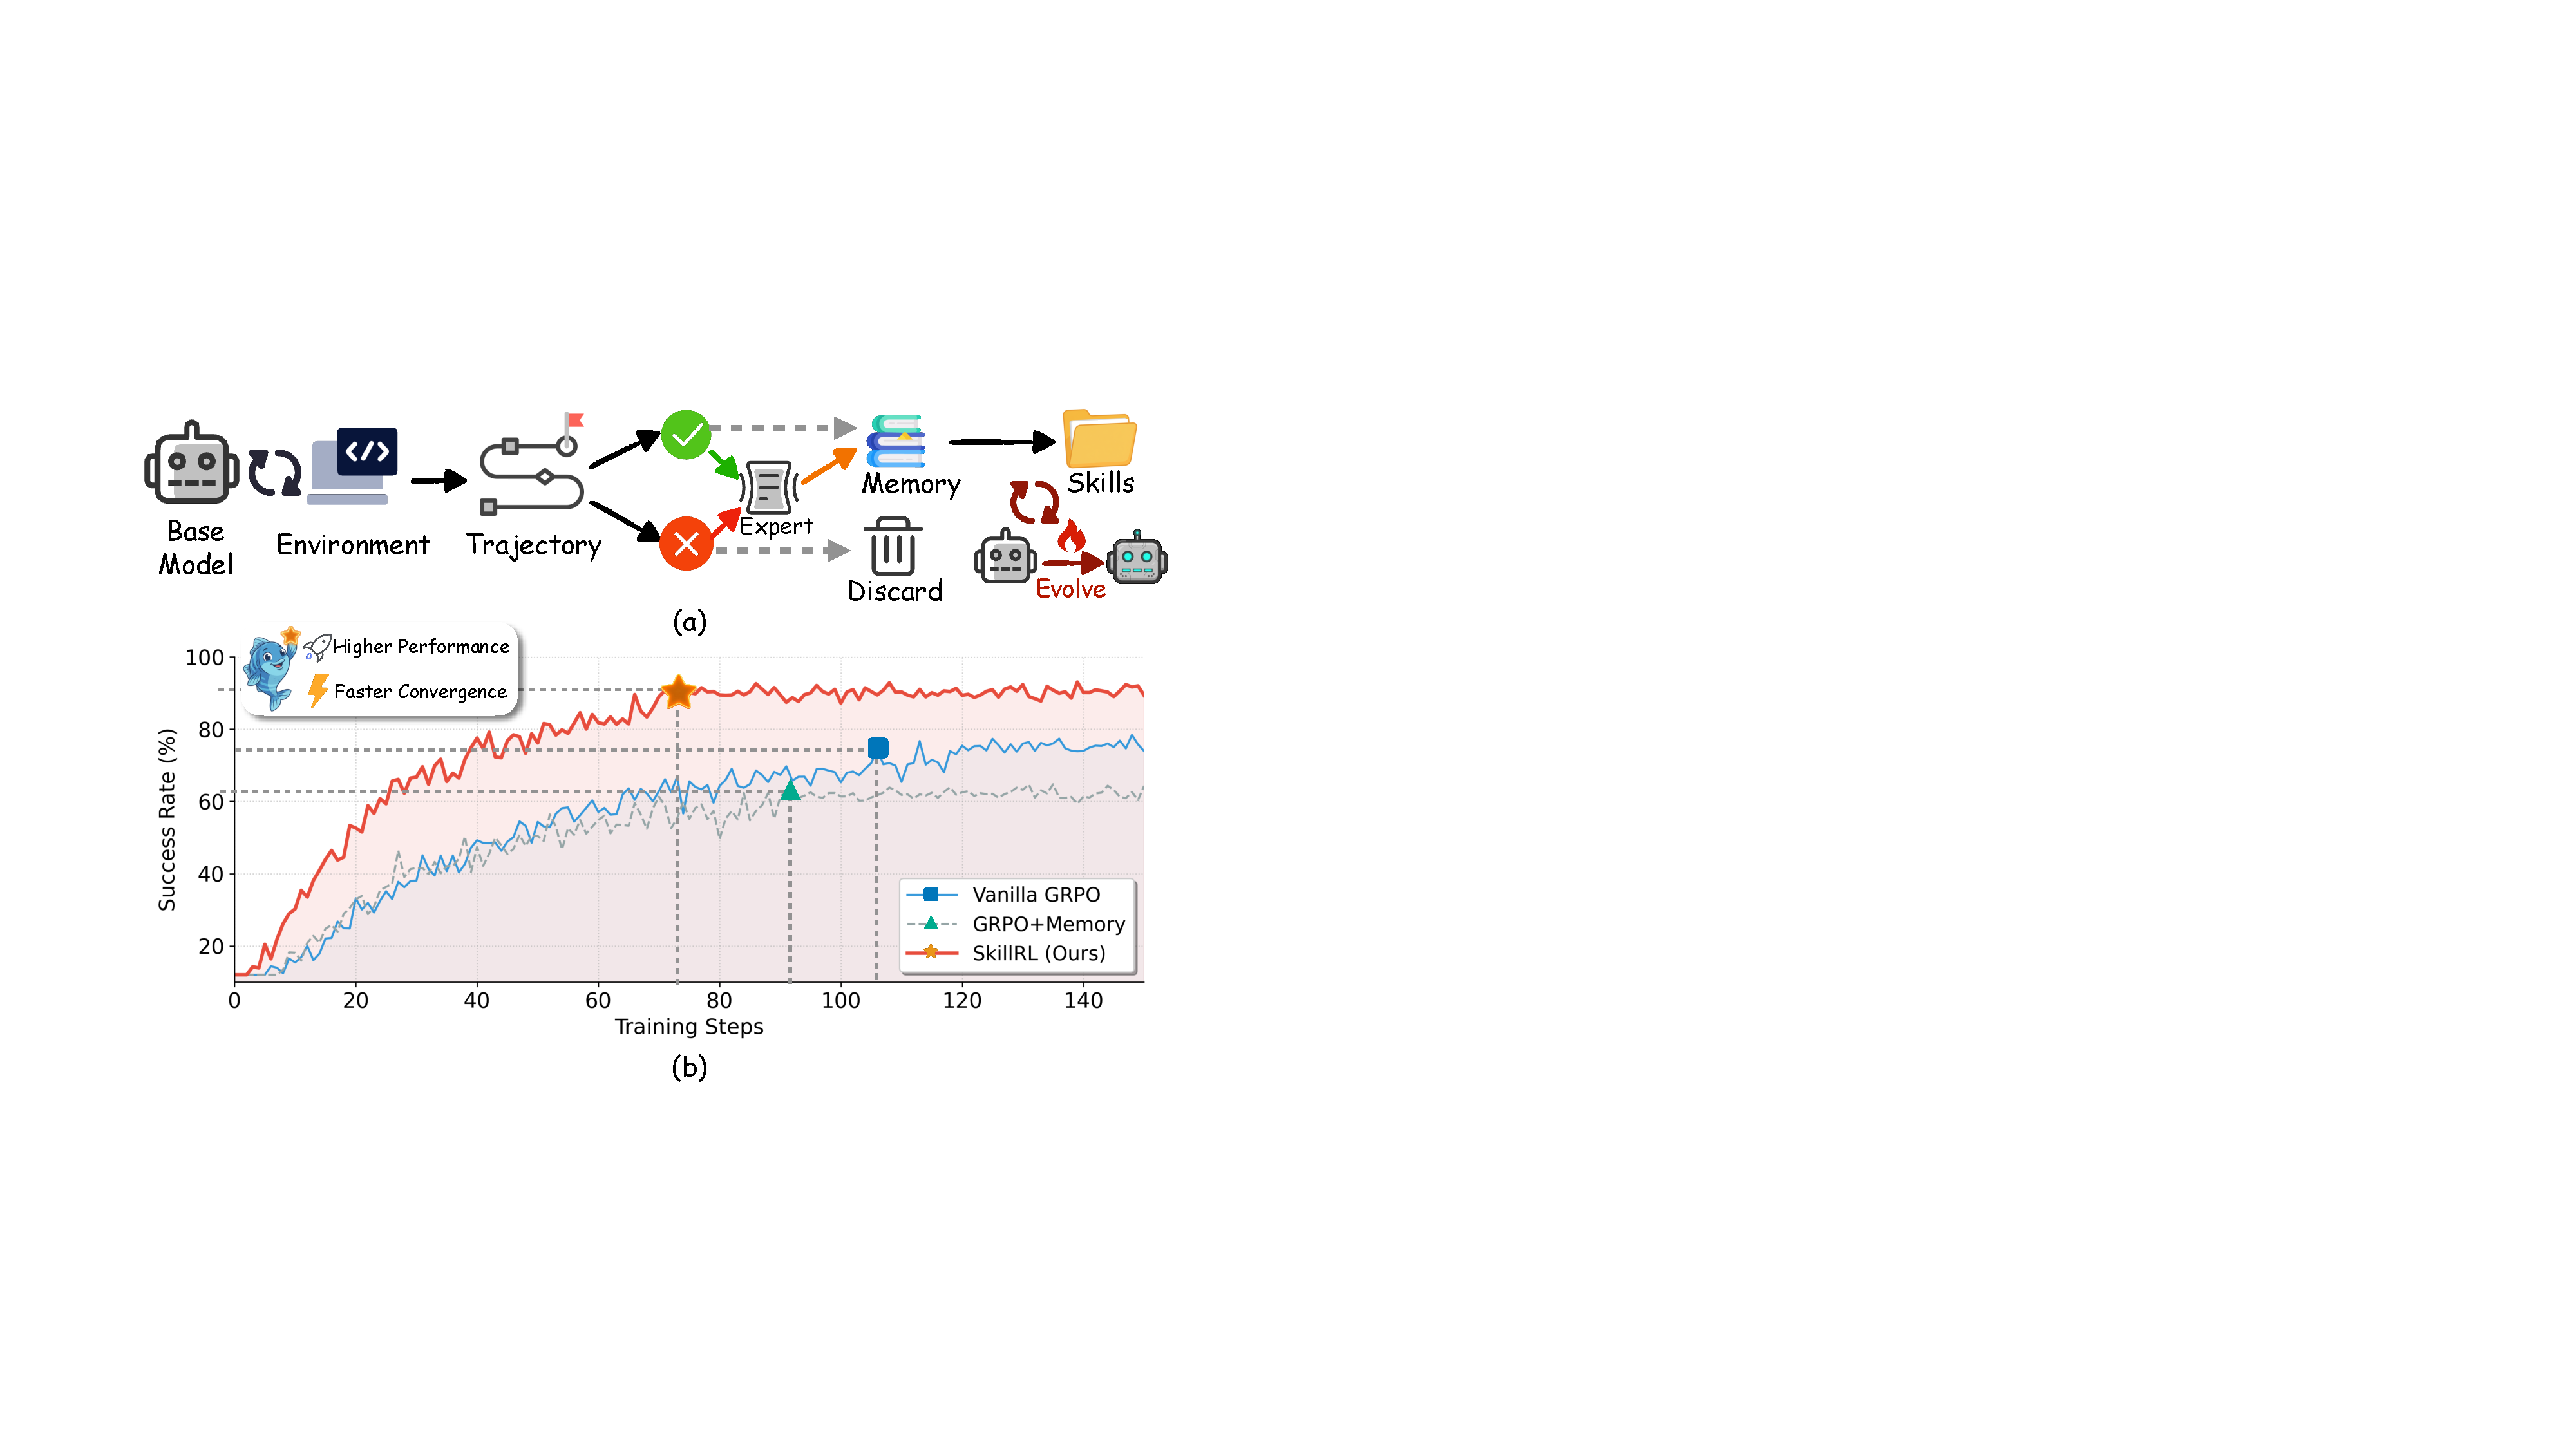
\includegraphics[width=0.45\textwidth]{asset/fig1.pdf}
    \caption{(a) Overview of the \method{} pipeline. Unlike previous methods (\textcolor{gray}{gray dashed lines}) that store raw trajectories and discard failures, \method{} employs an experience-based distillation mechanism to transform diverse experiences into structured skills. (b) Performance on ALFWorld validation set~\cite{shridharalfworld}. \method{} achieves faster convergence and superior success rates compared to vanilla GRPO and memory-augmented RL.}
    \label{fig:intro}
    \vspace{-1.5em}
\end{figure}


The existing memory-based methods for LLM agents primarily involve saving raw trajectories directly into external databases during the sampling process to serve as references for similar future tasks~\cite{shinn2023reflexion,zhao2024expel}. While intuitive, these raw trajectories are often lengthy and contain significant redundancy and noise~\cite{chhikara2025mem0}, making it difficult for the model to extract critical information. Recent work has attempted to compress trajectories and update the memory bank via online training~\cite{zhang2025memevolve,zhang2026memrl}, improving memory efficiency. However, these methods merely mimic past solutions and they fail to distill core principles or adapt the agent’s internal policy to leverage memory for guided decision-making. As depicted in the dashed flow of Figure~\ref{fig:intro}(a), such approaches often struggle with the trade-off between information density and noise, leading to sub-optimal performance or even degradation as shown in Figure~\ref{fig:intro}(b).

We argue that these approaches miss a crucial insight: effective experience transfer requires \emph{abstraction}. Human experts do not memorize every action in every situation; instead, they develop \emph{skills}~\cite{authropic3}, compact and reusable strategies that capture the essence of how to accomplish specific subtasks. Inspired by this observation, we propose \method{}, a framework that bridges the gap between raw experience and efficient policy improvement through automatic skill discovery and recursive skill evolution.

\method{} first introduces an experience-based skill distillation mechanism, which gathers diverse trajectories from environment rollouts and applies differential processing: successful episodes are preserved as demonstrations, while failed ones are synthesized into concise failure lessons to mitigate context noise. Secondly, we transform these experiences into a hierarchical skill library \skillbank, differentiating between \emph{general skills} for universal strategic guidance and \emph{task-specific skills} for task-level heuristics. This abstraction allows the agent to adaptively retrieve relevant skills during decision-making, significantly reducing the token footprint while enhancing reasoning utility. Lastly, \method{} incorporates a recursive skill evolution mechanism during reinforcement learning (RL), where the skill library is treated as a dynamic component rather than a static knowledge source. By analyzing failure modes after each validation epoch to generate new skills or refine existing ones, our approach ensures the skill library and the agent’s policy co-evolve, maintaining robustness as task complexity increases. As demonstrated in Figure~\ref{fig:intro}(b), \method{} achieves substantially faster convergence and higher asymptotic performance.

The primary contribution is \method{}, a framework that enables LLM agents to bridge the gap between raw experience and policy improvement through automatic skill discovery and recursive evolution. By distilling redundant trajectories into a hierarchical \skillbank, our method abstracts general and task-specific skills to guide decision-making efficiently. Furthermore, we introduce a recursive evolution mechanism that ensures the skill library and agent policy co-evolve during reinforcement learning. Empirical results on ALFWorld, WebShop, and seven search-augmented benchmarks demonstrate that \method{} achieves state-of-the-art performance with 15.3\% improvements, significantly outperforming current memory-based agent-tuning baselines in both task success and reasoning utility.
